\section{Differentialgleichungen}
Dieses Thema wird im Schwerpunktfach behandelt.
\section{Weitere Themen}
\subsection*{Integrationstechniken}
Wie wir gesehen haben, bilden die Stammfunktionen den Schlüssel zur Berechnung Integralen, die in vielfältigen Anwendungssituationen eine wichtige Bedeutung haben Umso einschränkender ist es, dass wir im Moment nur von ganz wenigen, einfachen Funktionen die Stammfunktion angeben können. Zum Beispiel:
\[
\int x\sqrt{x} \,dx = \frac{2}{5}x^{5/2} + c
\]
\[
\int e^x \,dx = e^x + c
\]
\[
\int \frac{1}{x} \,dx = \ln(|x|) + c
\]
\[
\int \sin(x) \,dx = -\cos(x) + c
\]

Sobald die Funktion ein klein wenig komplizierter wird, ist das Auffinden der Stammfunktion nicht mehr so einfach. Zum Beispiel
\[
\int x \cdot \cos(x) \,dx = ?
\]
In diesem Kapitel werden Sie Techniken kennenlernen, mit denen man in einigen Fällen die Stammfunktion bestimmen kann.

Diese Techniken haben gemeinsam, dass Sie gewissermassen eine Ableitungsregel umgekehrt anwenden. Eine dieser Techniken, haben Sie bereits kennengelernt: Die \emph{lineare Substitution}.

\begin{bsp}
    {Eine lineare Substitution}{}
    $$\int \cos(3x-1) \, dx = \sin(3x-1) \cdot \frac{1}{3} + C$$
\end{bsp}

Die linearen Substitution ist so etwas, wie die Kettenregel der Integration. Im Folgenden  werden wir uns mit Produkten von Funktionen befassen und eine Art ``Produktregel der Integration' kennenlernen.

\begin{LA}
    {Versuch und Irrtum}{}
    Finden Sie eine Stammfunktion von $f(x) = x\cdot \cos(x)$, indem Sie Kandidaten ausprobieren und laufend verbessern.
\end{LA}
 
\clearpage
\begin{satz}
    {Die partielle Integration}{}
    Sei $F$ eine Stammfunktion von $f$. Dann gilt
    $$ \int f(x)\cdot g(x) \, dx = F(x)\cdot g(x) - \int F(x) \cdot g'(x) \, dx$$
\end{satz}

\begin{proof}
    
    \vspace*{3cm}
\end{proof}

\begin{bsp}
    {}{}
    $\int x\cdot \cos(x) \, dx = $
    \vspace*{2cm} 
\end{bsp}
\begin{bsp}
    {}{}
    $\int x^2 \cdot \cos(x) \, dx= $
    \vspace*{6cm} 
\end{bsp}

\begin{bsp}
    {}{}
    $\int \ln(x) \, dx= $
    \vspace*{4cm} 
\end{bsp}

\begin{bsp}
    {}{}
    $\int \cos^2(x) \, dx= $
    \vspace*{8cm} 
\end{bsp}
\begin{ueb}
    {}{}
    Im Buch auf Seite 161 und 162.
    Zusätzlich
    \begin{enumerate}
        \item Berechnen Sie den Inhalt der Fläche zwischen dem Graphen von $f(x) = (x-2)\cdot e^{0.5x}$, der $x$ Achse und der Geraden $g: \: x=0$.
        
        (Lösung 2.87)
        \item Das Kurvenstück der Funktion $f:\: x\mapsto xe^x$, das zwischen Nullstelle und Extremum liegt, rotiert um die $x$-Achse. Berechnen Sie das Volumen des Rotationskörper
        
        (Lösung 0.25)
    \end{enumerate}
\end{ueb}
\clearpage
\subsection*{Nicht-lineare Substitution}
Mit der linearen Substitution können wir die Stammfunktion von Funktionen der Form $f(ax+b)$ bestimmen. Man kann das auch so betrachten, dass wir Funktionen der Form $f(u(x))$ integriert haben, wobei $u(x)=ax+b$ eine lineare Funktion ist. In diesem Abschnitt möchten wir der Frage nachgehen, was passiert, wenn $u(x)$ nicht linear ist. Dazu betrachten wir zunächst die andere Richtung: die Ableitung. Sei $F(x)$ eine Stammfunktion von $f(x)$. Dann gilt nach der Kettenregel:
$$\left( F(u(x)) \right)' = f(u(x)) \cdot u'(x)$$
Das lässt sich auch so formulieren:
\begin{satz}
    {Nicht-lineare Substitution}{}
    Sei $F(x)$ eine Stammfunktion von $f(x)$. Dann gilt

\[
\int f(u(x)) \cdot u'(x) \, dx = F(u(x))
\]

\end{satz}

Diesen Satz kann man sich gut merken, wenn man die Schreibweise $\frac{d}{dt}$ für die Ableitung nach $t$ verwendet:

\begin{satz}
    {Substitution in Kurzform}{}
    \[
\int f(u) \frac{du}{dt} \, dt = \int f(u) \, du
\]

\end{satz}
So wird deutlich, woher der Name „Substitution“ kommt: Man ersetzt die Variable, nach der integriert wird.

Die Schwierigkeit in der Anwendung besteht darin, die Funktion $f(u)$ und $u(x)$ zu erkennen. Betrachten Sie das folgende 

\begin{bsp}
    {Wird in der Klasse ergänzt}{}
    \[
\int \frac{1-x}{\sqrt{2x-x^2}} \, dx = ?
\]
\end{bsp}
\clearpage
\subsection*{Nicht elementar integrierbare Funktionen}
Die erlernten Integrationstechniken erwecken vielleicht den Eindruck, dass zu jeder Funktion unter Zuhilfenahme einer geeigneten Technik eine Stammfunktion ermittelt werden kann. Das stimmt aber nicht ohne Weiteres. Um diese Aussage zu verstehen, führen wir den Begriff der elementaren Funktionen ein:
\begin{definition}
    {Elementare Funktionen - eine mögliche Definition}{}
    Eine Funktion heisst \emph{elementar}, wenn sie eine Verkettung von (endlich vielen) Polynom-, Potenz-, trigonometrischen, Exponential- und Logarithmusfunktionen ist.\footnote{Es gibt allerdings keine allgemeingültige, präzise Definition von elementaren Funktionen}
\end{definition}
Fast alle Funktionen, die wir bis jetzt betrachtet haben, gehören zu dieser Klasse von Funktionen. Das hat damit zu tun, dass wir Funktionen meist durch Ihre Gleichung angeben. Damit sind sie automatisch eine Summe, Produkt oder Verkettung der bekannten Funktionstypen und somit elementar. Hinzu kommt, dass auch die Ableitung einer elementaren Funktion wieder elementar ist. Beim Integrieren ist das nicht der Fall!
\begin{bsp}
    {eine Funktion, die nicht elementar integrierbar ist}{}
    $$f(x) = \frac{1}{2\pi} e^{-\frac{1}{2}x^2}$$
    \begin{center}
        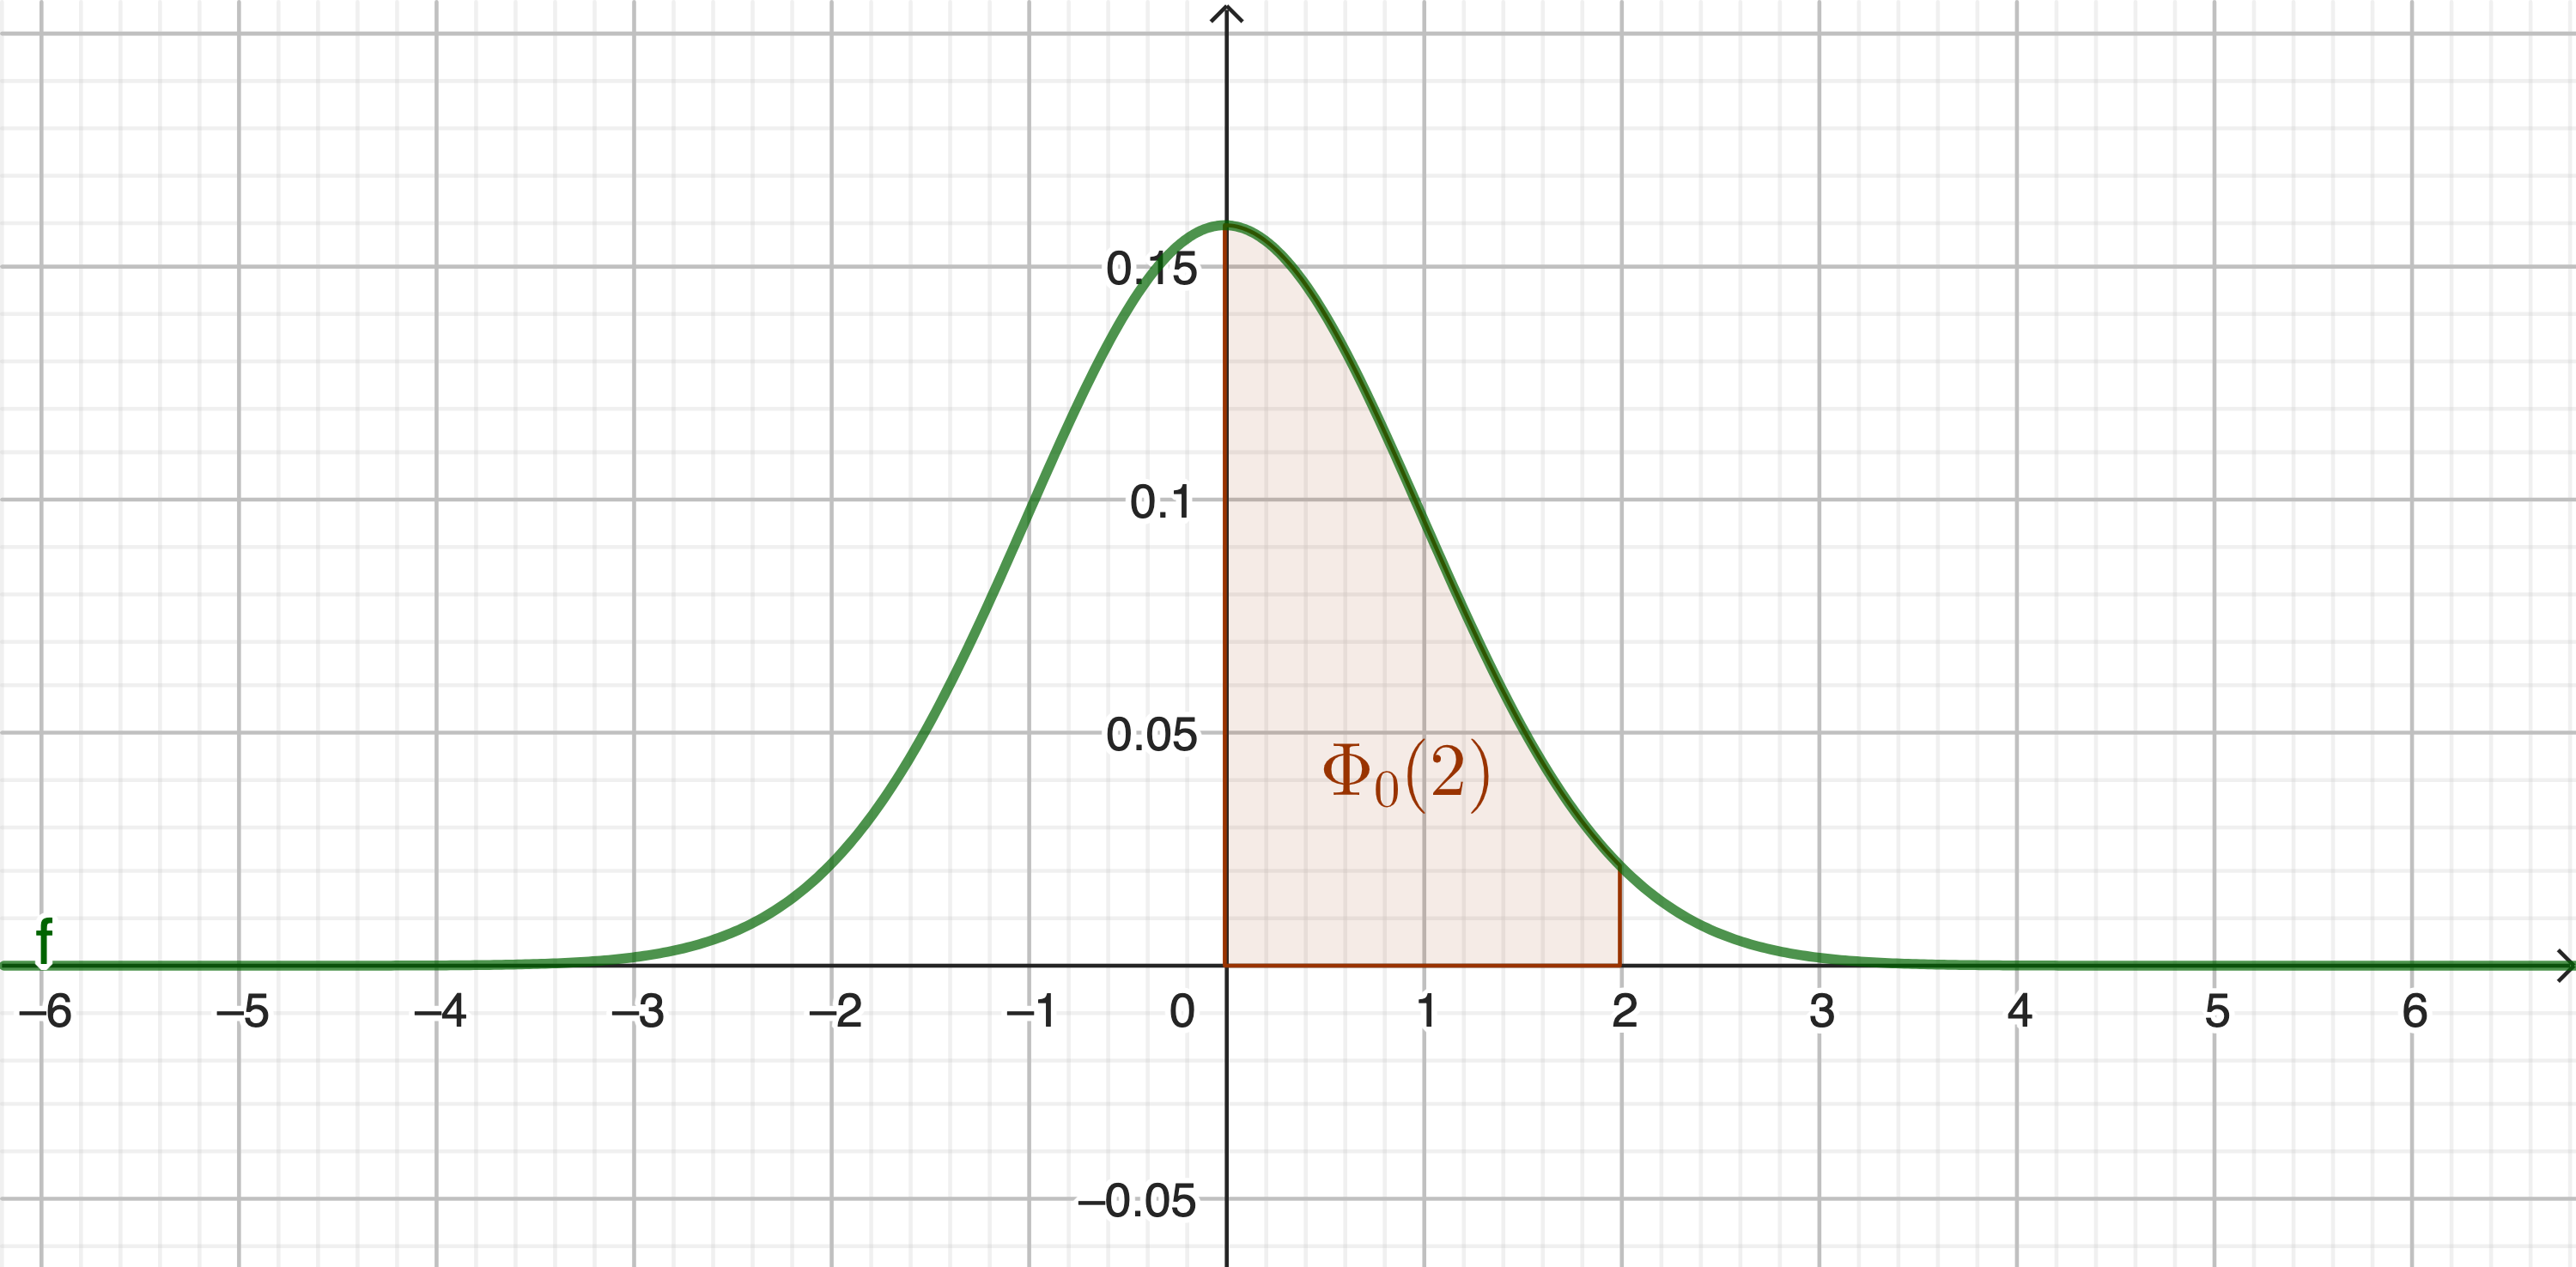
\includegraphics[width = 0.5\textwidth]{media/Glockenkurve.png}
    \end{center}

    Der Graph von $f$ wird auch Gauss'sche Glockenkurve genannt und ist in der Wahrscheinlichkeitsrechnung sehr wichtig. Die Funktion 
\[
\Phi_0 (t) = \int_0^t f(x) \, dx
\]
ist wohldefiniert, gehört aber nicht zur Klasse der elementaren Funktionen. Die Werte von $\Phi_0$ kann man näherungsweise bestimmen – zum Beispiel indem man die entsprechende Fläche durch die Ober- bzw. Untersumme approximiert.


\end{bsp}






